% !TeX encoding = UTF-8
% !TeX spellcheck = hu_HU
\documentclass[magyar,12pt,a4paper,final,titlepage]{report}

\usepackage[T1]{fontenc}
\usepackage[utf8]{inputenc}
\usepackage[usefilenames,DefaultFeatures={Ligatures=Common}]{plex-otf} %

\usepackage{babel}

\usepackage{url}
\usepackage[unicode,colorlinks]{hyperref}

\usepackage[acronym]{glossaries}

\usepackage{amsfonts,amsmath,amssymb} % Mathematical symbols.
\usepackage{booktabs} % For publication quality tables for LaTeX
\usepackage{graphicx}
\usepackage{pdfpages}
\usepackage{listings}

\usepackage{anysize}
\usepackage{sectsty}
\usepackage{setspace} % For setting line spacing
\usepackage{geometry}

\usepackage[amsmath]{ntheorem} % Theorem-like environments.

\usepackage{subcaption}

\theoremseparator{.}
%\theoremprework{\bigskip\hrule\medskip}
%\theorempostwork{\hrule\bigskip}
\theorembodyfont{\upshape}
\theoremsymbol{{\large \ensuremath{\centerdot}}}
\newtheorem{property}{Tulajdonság}

\pagestyle{plain}
\marginsize{25mm}{25mm}{15mm}{15mm}

\title{Fordítóprogramok készítése\\
BMEVIIIML10 --- Önálló laboratórium 1\\
Beszámoló}
\author{Bodor András}

\def\hyph{-\penalty0\hskip0pt\relax} % Kötőjeles szavak elválasztásának engedélyezése
\hyphenation{
    a-mely-ek
    szak-ter-ü-let
    év-en-te
    }


\definecolor{inline-code-color}{HTML}{086834}
\def\inlcode#1{{\color{inline-code-color}\tt #1}}

\def\pl{pl.\ }
\def\ld{ld.\ }
\def\un{ún.\ }
\def\textlambda{λ}

\bibliographystyle{IEEEtranSA}

\frenchspacing

\setlength{\parindent}{2em}
\setlength{\parskip}{0em}
\frenchspacing

\input glossary

\definecolor{lightgray}{rgb}{0.95,0.95,0.95}
\lstset{
    basicstyle=\scriptsize\ttfamily, % print whole listing small
    keywordstyle=\color{black}\bfseries, % bold black keywords
    identifierstyle=, % nothing happens
    % default behavior: comments in italic, to change use
    % commentstyle=\color{green}, % for e.g. green comments
    stringstyle=\scriptsize,
    showstringspaces=false, % no special string spaces
    aboveskip=3pt,
    belowskip=3pt,
    backgroundcolor=\color{lightgray},
    columns=flexible,
    keepspaces=true,
    escapeinside={(*@}{@*)},
    captionpos=b,
    breaklines=true,
    frame=single,
    float=!ht,
    tabsize=2,
    literate=*
    {á}{{\'a}}1	{é}{{\'e}}1	{í}{{\'i}}1	{ó}{{\'o}}1	{ö}{{\"o}}1	{ő}{{\H{o}}}1	{ú}{{\'u}}1	{ü}{{\"u}}1	{ű}{{\H{u}}}1
    {Á}{{\'A}}1	{É}{{\'E}}1	{Í}{{\'I}}1	{Ó}{{\'O}}1	{Ö}{{\"O}}1	{Ő}{{\H{O}}}1	{Ú}{{\'U}}1	{Ü}{{\"U}}1	{Ű}{{\H{U}}}1
}


\begin{document}
    \maketitle

    \tableofcontents
    \newpage

    \onehalfspacing

    \chapter{A feladat leírása}

    \section{Feladatkiírás}\label{sec:feladat}

    \sloppy % külső ,,kódot'' nem próbálunk meg jól formázni

    A szoftverfejlesztést nagyban megkönnyíthetik az olyan eszközök, amelyek leveszik a programozó válláról a mechanikusan végrehajtandó feladatokat (\pl JPA entitások készítése, REST interfész generálása, DTO objektumok definiálása, stb.). Sokszor egy egyszerű, a problémakörhöz közelebb álló szakterület\hskip0pt--specifikus programnyelv (domain--specific language) hatékonyabb munkát biztosíthat, mint az általános programnyelvek segítségével elvégezni a feladatot.

    A téma során a hallgató feladata egy egyszerű programnyelv definiálása, majd ehhez egy fordítóprogram írása. A fordítóprogram készítése során front-end (\pl Xtext, ANTLR4) és back-end (\pl LLVM) eszközök is használhatók.

    \fussy

    \section{Motiváció}\label{sec:motiv}

    A feladat célja, egy olyan nyelv elkészítése, amelyiket lehetséges lesz a későbbiekben továbbfejleszteni egy általános C és C++ kódbázisokban mintázatokat kereső eszközzé.
    Azon keresztül pedig, hogy kódrészleteket lehet keresni egy adott kódbázisban, különböző módon lehetséges reagálni.
    Az egyik felhasználási lehetőség lehet házi feladatok ellenőrzésénél egyes tárgyak elvárásainak teljesülését vizsgálni.
    De például ha dokumentáció nem a kódban található, akkor annak a megléte a megfelelő külső fájlban is ellenőrizhetővé válik, a kíván művelet implementálásával.

    Felmerülhet a kérdés, hogy miben más ez/miben különül el, a már meglévő és akár nyílt forráskódú, akár kommersz statikus analízist végrehajtó eszközök széles tárházától.
    Ezek az eszközök nagyszerűen tudnak nyelv--specfikikus hibás idiómákat (\pl virtuális destruktor hiánya egy ősosztályban C++-ban), és általános code--smelleket (\pl túlságosan nagy osztály/függvény) megkeresni és jelezni a fejlesztők felé.
    Sok esetben a kedvenc fejlesztőkörnyezetünkben léteznek hozzájuk megfelelő bővítmények, amelyek a hibás/hibásnak vélt kódrészleteket aláhúzzák, így kódolás közben, valós időben is tájékoztatnak a nem feltétlen szerencsés kódrészletekről.

    A végső cél projekt az előbb leírt gondolatnak egy általánosított változatát kívánja megvalósítani.
    Az elérhető statikus analízis eszközök nagy része előre konfigurált mintázatokat keresnek egy-egy kódbázisban, és új felvételéhez a fejlesztőknek azt az eszköznek megfelelő módon bele kell illeszteniük, amit a következő verziószám alatt elérhetővé lehet tenni.
    Így működik a C és C++ nyelvekhez az LLVM projekt gondozásában készült ,,{\tt clang-tidy}''.~\cite{llvm_project_getting_nodate}
    Esetlegesen, ha mégis támogatják saját minták felvételét, akkor sem garantált, hogy tetszőleges kód futtatását lehetővé teszik azon mintázatok megtalálásának hatására.

    Itt ki kell emelni, hogy egyes nyelvekhez (\pl Ruby) léteznek ennél jóval inkább dinamikus statikus analízis eszközök (a Ruby nyelvhez konkrétan a RuboCop \cite{rubocop_project_development_nodate}, amelyik dinamikusan tud betölteni ellenőrző ,,cop'' (rendőr) osztályokat egy--egy projektben saját célokra), de ilyenek eszközről nem tudok a C és C++ nyelvek ökoszisztémájában.

    \section{Általános elvárások}

    Az előzőek ismeretében ebben a fejezetben olyan követelményeket/elvárásokat rögzítek, amelyet a nyelv jövőbeli használatát hivatottak lehetővé tenni a bemutatott feladatra.

    \begin{property}\label{prop:uncompiled}
        Fordítás nélkül futtatható.

        \noindent A nyelvnek lehetőség szerint nem fordítottnak kell lennie, hogy ne kelljen a különböző ellenőrzések fordításával foglalkozni ahhoz, hogy egy--egy projekt le tudjon ellenőrizni valamilyen saját elvárást a kódjában.
        Ez a tulajdonság hasznossá válik pipeline-okban való használat esetén is, mert nem szükségelteti, hogy egy külön lépést definiáljunk csak az ellenőrzések fordítására.
        Ennek az elvárást teljesíti egy egyszerű interpreter de egy komplett \gls{JIT} rendszer is.
        Az alább leírt megvalósítás az utóbbit használja.
    \end{property}

    \begin{property}\label{prop:dynamic}
        Dinamikusan típusos

        \noindent A mai napig heves (hit)vita folyik a statikusan és dinamikusan típusos nyelveket támogató táborok között az egyik másiknál jobbnak létéről.
        Klasszikusan a különböző interpretált \un ,,script nyelvnek'' kategorizált nyelvek utóbbi csoportba tartoznak, \pl Perl, Ruby, Python, Tcl, és a különböző Shell nyelvek (Bash, ZSH, tcsh, CMD.EXE), míg a fordított nyelvek inkább statikus típusokkal dolgoznak, \pl C, C++, Java, C\#, Rust.
        Ennek alapja a nyelvek alapvető célja: ha rövid ,,scripteket'' kíván valaki írni, akkor általában valami rövid, egyszerű logikát megvalósító egyszer-egyszer magában lefuttatott kódra gondolunk, aminek általában nem elsődleges célja a hosszú távú karbantarthatóság, vagy pusztán a kód kis mérete miatt ez nem számít nehézségnek, így a típusok nem számítanak annyira hasznosnak.
        Ennek a gondolatmenetnek következményeként, egy vélhetően rövid ellenőrző ,,script'' esetén a dinamikus típusok megkönnyítik a gyors fejlesztést, hogy a megfelelő kódrészleteket meg tudjuk keresni, és valamit tudjunk velük csinálni.
    \end{property}

    \begin{property}\label{prop:dsl-friendly}
        Erős beágyazott \gls{DSL} támogatás.

        \noindent Mivel a nyelven elsődlegesen különböző kódrészleteket szeretnénk megkeresni, és azokat megtalálva valamilyen reakciót lefuttatni, így két lehetőség adódik: a nyelv szintaktikájába alapból beépíteni a keresés lehetőségét vagy egy olyan általános lehetőséget biztosítani, amin keresztül lehetséges lesz, hogy a nyelven belül kerüljön ez definiálásra.
        Az első megoldásra példa az AWK nyelv, amelyikben a különböző regexek és a sikeres találatukkor lefutott kód erősen része a nyelv szintaktikájának.

        Mivel itt elsődlegesen a C és C++ nyelvek \gls{AST} alapú leírásában próbálunk keresni, így a második lehetőség kényelmesebb eredményt nyújthat: ezek a nyelvek gyakran és előre várható periodicitással változnak (\textasciitilde 3~évente), így elég dinamikusságot kell kezelni a kereső szintaktikában.
    \end{property}

    \begin{property}\label{prop:easy}
        Egyszerűen érthető egy C vagy C++ fejlesztőnek.

        \noindent Elsődlegesen C és C++ programozók azok, akik C vagy C++ kódban szeretnének kódrészleteket megkeresni, így a megvalósított nyelvnek legalább szintaktikában jó lenne hasonlítani ezekre a nyelvekre, hogy ne növeljük meg fölöslegesen az értelmezést, vagy a
        kód írásának befektetett energiaigényét.
        Bár ennek a tulajdonságnak a legegyszerűbb kielégítése C vagy C++ használata lenne, az előző tulajdonságokban leírtak miatt ez nem egy ideális választás.
    \end{property}

    \chapter{A nyelv ismertetése}

    \section{A nyelv áttekintő leírása}\label{sec:c4}

    Az előző tulajdonságok alapján megalkotott nyelv leírása következik.
    Magas szinten, egy olyan nyelvet definiálok, amelyik funkcionális, erősen immutábilis, dinamikusan típusos, és nagyon dinamikus a szintaktikáját tekintve.

    Ezeknek a tulajdonságoknak nagy része megfelel és direkt következménye az előző részben definiált elvárásoknak.
    A funkcionális, immutábilis nyelv választása azonban nem egyértelmű: a klasszikus könnyen futtatható, dinamikus nyelvek nagy többségben egyszerű procedurális paradigma szerint működnek \ld Tcl, shell nyelvek, esetleg utólagosan különféle módon objektum--orientált támogatást kaptak ilyen \pl a Perl.
    Ezekben a nyelvekben látszik, hogy az egyszerű procedurális paradigma nagyon kevés segítséget biztosít a programozónak a kód megírása közben: nagyrészben imperatív kódot kell, egymást hívó procedurák sorozataként modellezni, magasabb szintű absztrakciók nyelvi támogatottsága nélkül.
    (\ld C-ben (nem ,,script'' nyelv, de procedurális) objektum--orientált programozáshoz manuálisan kell megvalósítani a virtuális függvénytáblát.)

    A megvalósított nyelvnek a funkcionális irányzatot választottam tehát a procedurális és objektum orientált helyett.
    Az előbbi megközelítés nagyon kevés támogatást ad a programozónak, míg az utóbbi nagy mennyiségű extra kódot igényelhet (osztályok/metódusok definiálása, példányosítások) egy ilyen egyszerű célú kódot támogató eszköz számára, ami elsődlegesen nagy rendszerekben mutatkozik előnynek, nem pár száz soros fájlok írásakor.

    Megjegyzendő még az elterjedt paradigmák közül a logika alapú programozás (\ld Prolog gyakorlatilag egyeduralkodóként), ami nagyon sok programozónak kifejezetten idegen, így fölöslegesen nagy nehézséget állít azok elé, akik egy egyszerű ellenőrzést kívánnak csak megvalósítani a programjukhoz.
    Egy bár funkcionális, de kevésbé szigorú (dinamikus) típusrendszerű nyelv az elgondolás szerint nem rendelkezik ennyire kiemelkedően ezzel a problémával.

    \section{A nyelv családja és ismerősei}

    ,,Minden egy függvényként kerülhet definiálásra.''
    Ez a gondolat a LISP család tagjaként is tekinthetővé teszi ezt a nyelvet, és míg lehetőség van LISP jellegű kódot írni, nem ez az elsődleges cél.
    Magában a LISP másolásával pár nehézség lép fel, így a következőkben kifejtésre kerül, hogy helyette milyen módon kerül ez megvalósításra.

    \paragraph{LISP család}
    A LISP az egyik legöregebb programozási nyelvek közé tartozó funkcionális nyelv.
    Kiemelkedő jellegzetessége az \un szimbolikus kifejezés (\gls{sexpr}; innentől \gls{sexpr}) (eredetileg \cite{mccarthy_recursive_1960}), amelyik a kód elkülönülő kinézetét adja.
    Minden kifejezés egy {\tt (fv param1 param2...)} formátumban áll elő, \pl \inlcode{(+ 1 1)}.
    Ez lehetővé teszi a nagyon egyszerű feldolgozást, hiszen a zárójelek és \gls{prefix} formájában megadott függvényhívás egyértelművé teszik a szöveg jelentését komolyabb számítások nélkül is (ellenben \pl egy \gls{infix}, amit a matematikából megszoktunk $1 + 1$).
    \vskip.3cm

    A LISP nyelvek az egyik legdinamikusabb szintaktikát tudják biztosítani, ami \aref{prop:dsl-friendly}.~tulajdonság szempontjából nagyon kedvező.
    Egy probléma adódik, miszerint a LISP nyelvek nem számítanak annyira elterjedtnek, mint a C vagy C++ nyelvek, így sok C és C++ programozó van, aki nem tud és valószínűleg nem is akar LISP kódot írni, ha ezt meg lehet oldani.
    Ez szembe megy \aref{prop:easy}.~tulajdonságban leírtakkal, így nem lenne ideális választás egy LISP szintaktikai szintű megvalósítása.

    Egy kompromisszumot kell megállapítani a LISP általánossága és a megszokott C jellegű szintaktika között.
    Hasonlóan, mint a Tcl nyelv amelyik LISP jellegű szemantikával dolgozik egy C jellegű szintaktikát felhasználva.
    A Tcl azonban erősen procedurális nyelv, egy kis OO támogatással, amelyiket az évtizedek alatt összeszedett, így nem illeszkedik a funkcionális gondolatmenetre.
    Ebben a nyelvben a ,,minden procedúra'' gondolatmenet mutatkozik meg, így még az egyszerű elágazás (\inlcode{if}) is újradefiniálható a megfelelő procedúra definiálásra használt szintaktikával.
    Ennek a gondolatmenetnek a felhasználásával mutatom be a következő szakaszban az itt definiált nyelvet.

    \section{A nyelv felépítése}

    Nincs külön belépési függvény, a kód, ahogy megtalálható a fájlban fut.
    Ez hasonlít sok másik interpreterrel futtatott nyelvre.

    Az előző rész elején említetteknek megfelelően az következne, hogy minden egy függvény.
    Egy kivétel azonban van, amivel a Tcl jobban megközelítette az általánosságot: a \inlcode{let} nyelvi elemként kerül megvalósításra, ellenben a Tcl \inlcode{proc}cal.
    Ez a feldolgozás egyszerűsítését hivatott előidézni, mert így a \inlcode{let} kódját annak feldolgozása közben el tudjuk különíteni más \glspl{token}étől, ami lehetővé teszi, hogy egyáltalán értelmezni tudjuk a nyelvet.

    \subsection{Literálisok}

    Egyszerű literálisok a sok nyelvben megszokott szintaktikával létrehozhatóak:
    \begin{description}
        \item[Egészek] {\tt 42,~1234}
        \item[Tizedes törtek] {\tt 4.2,~0.0}, nem lehet lehagyni az egyik részét sem a számnak, tehát {\tt .2,~2.} nem érvényesek.
        \item[Szöveg] {\tt "szöveg"}, ez lehet több soros is.
    \end{description}

    \noindent Az utolsó literális fajta a blokk, amelyről \aref{subsec:block}.~szekcióban lesz szó.

    \subsection{Változók}

    Egy programozási nyelv bevezetésekor sok esetben a változókkal lehet kezdeni, mert elég egyszerűek azoknak is akik még nem programoztak, akik meg már tudnak programozni rögtön tudják hova kötni a már ismert nyelveik közé.
    Jelen esetben azonban fel kell ismerni valamit.
    A változók is igazából függvények.
    Mivel immutábilis értékekről van szó (leszámolva pár nem \gls{pure} függvényt, amelyik be van építve IO műveletekre), így minden változó értelmezhető egy nulla aritású (nulláris) függvényként, amelyik mindig a definiálásakor kapott értéket adja vissza.
    Ennek felismerésével nem kell külön megvalósítani a változókat, elég tisztán a függvényeket általánosan használhatóvá tenni nulla paraméter estén is.

    Megemlítendő, hogy ez a szemantika eltér a LISP-es vagy Lambda kalkulusos értelmezéstől, amelyekben a nulla paraméteres függvények nem értelmezettek.
    Ez utóbbi esetében egyértelműen látszik, hiszen minden \textlambda--absztrakció pontosan egy paramétert vár.
    Előbbi esetben kicsit bonyolultabb, de összességében egyszerű a levezetés: egy függvényhívás szintaktikája nulla bemenő paraméterrel a következő: {\tt (f)}.
    Ez azonban $(f) \equiv (f . \mathrm{NIL}) \equiv (f . ())$, ami tehát azt jelenti, hogy $f$ itt egy speciális egyedi értéket kap paraméternek, amelyikből csak pontosan egy van.
    Egyes nyelvekben ezt ,,Unit''-nak hívják.

    \subsection{Függvények}

    Minden függvényt a \inlcode{let} kulcsszóval lehetséges bevezetni.
    Egy függvényhez szükséges megadni a nevét, aritását és a hozzá tartozó törzset.
    Ebből az első két tulajdonságot a Prolog jellegű funktor jelöléssel lehetséges megadni: egy név egy perjellel elválasztva egy nemnegatív egész számtól, ami az aritás.
    Ezt hívjuk egy {\sl szimbólumnak}, és a perjel egyik oldalán sem lehetséges szóközt hagyni.
    Ha az aritás nulla (egy változót definiál a \inlcode{let} kifejezés), akkor a {\tt /0} elhagyható.
    Példa függvények definiálásra látható \aref{lst:funs}.~listában.

    \begin{figure}
        \begin{lstlisting}[gobble=12,language=haskell]
            let var 1
            let var1/0 var
            let fn/1 { |x|
                print "fn"
                var + x
            }
            let fn2/2 { |a b| (fn a) - b }
        \end{lstlisting}
        \caption{Példa változók és függvények definiálására}\label{lst:funs}
    \end{figure}

    A függvény törzsének pontosan annyi szabad paramétertől kell függenie, amekkora az aritása a függvény szimbólumának.

    \subsection{Blokkok}\label{subsec:block}

    Egy függvény törzsében legtöbbször szükséges megadni egyéb másik függvényhívásokat, hogy a működést a kívánt módon meghatározzuk.
    Ehhez sokszor több, mint egy másik függvény hívására van szükség.

    Egyes függvénytörzsek megadásához szükség van bevezetni ideiglenes, csak a függvényen belül értelmezett változókat (nulláris függvényeket), amelyek a szabad változóként műküdnek.
    Informatikai nomenklatúrában a függvények paramétereit meg kell tudni nevezni.

    Mind kettő problémára a blokkok adnak megoldást: ezek olyan kapcsos zárójelekkel (\{\}) körbefogott függvényhívások sorozatai, amelynek az értéke az utoljára kiértékelt függvényhívás.
    Ilyen értelemben ezek is függvényként viselkednek, hiszen van valahány bemenetük és garantáltan adnak vissza egy másik értéket.
    Ebből a tulajdonságból már következik a több függvény hívásából adó problémára a megoldás.
    Szabad változókat pedig a Ruby szintaxisához hasonló módon a blokk legelején pipe karakterekkel (|) behatárolva lehetséges megadni, azonban szóközökkel elválasztva.
    Mind kettő használatra látható példa \aref{lst:funs}.~listában.

    \paragraph{Az üres blokk}
    Az üres blokk egy speciális egység, amelyik más nyelvek \inlcode{null}, \inlcode{nil} vagy {\tt ()} elemeinek feladatait látja el.
    Azonban ezektől a megvalósításoktól egy különbsége van: egy teljes értékű blokk.
    Meglepetést nem okozva, nulla paramétere van, de az előzőek alapján minden esetben vissza kell adnia egy értéket, mert a blokkok függvényként viselkednek.
    Így visszaadja saját magát, az üres blokkkot.

    \subsubsection{Operátorok}

    Az operátorok olyan speciális függvények, amelyek csak szimbólum karakterekből állnak és vagy \gls{prefix}, vagy \gls{infix} formájában jelennek meg a kódban.
    Ennek megfelelően vonatokzik rájuk egy megkötés: csak egy vagy kettő paraméterük lehet.
    Az, hogy melyik, az a pre-, vagy infix tulajdonságukat határozza meg.

    Az \gls{infix} formájú operátorok esetében van még két tulajdonság, amit figyelembe kell venni: a \gls{precedence} és \gls{associativity}\footnote{Nem a matematikai értelemben kell itt értelmezni, hanem a nyelvek definiálásnál használt értelmezésben. \ld szójegyzék a definícióért.}.
    Asszociativitásból lehet \inlcode{left} vagy \inlcode{right} a bal és jobb asszociativitásért, míg precedencia egy $0$-tól $10$-ig tartó egész érték bármelyike lehet.
    Minél magasabb a szám, annál hamarabb kerül kiértékelésre.

    Mivel az operátorok is függvények, így definiálni a \inlcode{let} kulcsszóval lehetséges:
    az operátor zárójelek között aritásával megadva, majd az asszociativitás és precedencia tulajdonsága, végül a megszokott törzs.
    Példa található \aref{lst:ops}.~listában.

    \begin{figure}
        \begin{lstlisting}[gobble=8,language=haskell]
        let (+>)/2 left 2 { |a b| ... }
        let (?)/1 { |x| ... }
        1 +> 2
        ?1
        \end{lstlisting}
        \caption{Példa operátorok definiálására és használatára}\label{lst:ops}
    \end{figure}

    \subsubsection{Logikai kifejezések}

    Feltűnő lehet a \inlcode{true} és \inlcode{false} kulcsszavak/literálisok hiánya.
    Ez azonban könnyen feloldható: az üres blokk, mint ahogy az előzőekben bevezetésre került számít ,,hamis'' értéknek, minden más ,,igaz''.
    Bár ezt a nyelv nem kényszeríti ki, a beépített logikai értékeket használó függvények ezt a konvenciót használják.

    Könnyedségként azonban, két nulláris függvény is definiált: \inlcode{true/0} és \inlcode{false/0}.
    Ezek a nevüknek megfelelő logikai értéket adnak vissza, így a kódban jobban átlátható lesz, mint üres blokkok (hamis) vagy fura konstansok (igaz) használatával.

    \subsection{Lustaság}

    Egyes (funkcionális) nyelvek \un \gls{lazy} kiértékelést alkalmaznak.
    Ilyen például a Haskell.
    Ez azt jelenti, hogy egy függvényhívás, változó kötés stb.\ addig ténylegesen nem történik meg, amíg a program olyan lépést nem hajt végre, amelyik szükségessé teszi annak a kiszámítását.
    Példa erre a viselkedésre látható \aref{lst:lazy-haskell}.~listázában.

    Mivel minden függvény, így az if és egyéb nyelvi szerkezetek is.
    Emiatt szükség van annak a lehetőségére, hogy úgy vegyen át egy--egy függvény paramétert, hogy az ne értékelődjön ki.
    Az előbb említett if erre egy jó példa: ha az első paramétere (logikai feltétel) igaz akkor a harmadik paraméterét nem kell/szabad kiértékelni.
    Analóg módon a hamis esetben a második paraméterrel.
    Ennek megoldására jó lehetőséget nyújt az általános \gls{lazy} kiértékelés minden paraméterben.
    Látható ennek eredménye egy, a Haskell kóddal analóg példában \aref{lst:lazy-c4}.~listázában.

    \begin{figure}
        \hfil
        \hskip12pt
        \begin{subfigure}[h]{.41\linewidth}
            \begin{lstlisting}[numbers=left,language=haskell,gobble=16]
                -- nagyon nem idiomatikus Haskell kód, lustaság példa
                bar = do
                    putStrLn "bar"
                    return 42

                foo x = do
                    putStrLn "foo"
                    x

                main = do
                    foo bar
                    putStrLn "main"
            \end{lstlisting}
            \caption{Lusta Haskell kód}
            \label{lst:lazy-haskell}
        \end{subfigure}
        \hskip1cm
        \begin{subfigure}[h]{.22\linewidth}
            \begin{lstlisting}[numbers=left,language=haskell,gobble=16]
                let bar {
                    println "bar"
                    42
                }
                let foo/1 { |x|
                    println "foo"
                    x
                }
                foo bar
                println "main"
            \end{lstlisting}
            \caption{Lusta C4 kód}
            \label{lst:lazy-c4}
        \end{subfigure}
        \hskip.4cm
        \begin{subfigure}[h]{.13\linewidth}
            \begin{lstlisting}[gobble=12]
            foo
            bar
            main
            \end{lstlisting}
            \caption{Kimenet}
        \end{subfigure}
        \hfil
        \caption{Lustaság példa}
    \end{figure}

    \chapter{Megvalósítás}\label{sec:impl}

    Ebben a fejezetben részletezésre kerül az előző fejezetben ismertetett programozási nyelv megvalósítása.
    Elsőként a szöveg értelezésére térek ki, majd a bináris generálásának folyamatára.

    \section{A lexikális feldolgozás}

    A lexikai feldolgozás saját megvalósítás.
    A PCRE2 könyvtárat \cite{philip_hazel_pcre_2015} és annak a megfelelő \gls{JIT} támogatását használja, hogy a lehető leggyorsabban \glspl{token}re tudjuk bontani a szöveget.\footnote{Jelenleg a konstans szövegeket is reguláris kifejezéssé alakítva kezeli a c4c. Ez nem optimális, de a megvalósításban megvan a hely egy megfelelő szöveg illesztőnek.}
    Minden token egy saját típusként jelenik meg, a lexikai elemző pedig ezeknek egy \inlcode{std::variant} objektumba csomagolt értékét generálja.

    Egy fontos részlet, hogy a mind a lexikai elemző, mind az értelmező elkerüli a memóriafoglalást ahol csak lehetséges, hogy ezzel is hatékonyabb legyen az értelmezés folyamata.
    Ehhez egy fájl feldolgozása a \gls{memory-mapping} művelettel kezdődik.
    Innentől minden \gls{token}, és minden \gls{AST} csúcspont, amelyik a forrásfájl szövegére hivatkozik, csak pointert tárol erre a nagy memóriára, ezzel elkerülve az egyes (rövid) szövegdaraboknak való külön memória foglalást.

    \section{Az értelmező}

    Az értelmező nagy részben megszokott módszereket alkalmaz.
    Egy manuálisan megvalósított, legtöbb részében szokásos LL(1) algoritmus szolgál az alapjául.
    Az érdekesnek vélt részeit az alábbi alszekciók mutatják be.

    \subsection{Hibaüzenetek}

    Az egyik legfontosabb tulajdonsága egy fordítónak felhasználói szempontból, a helyesség mellett, hogy a generált hibaüzenetek érthetőek és jól olvashatóak legyenek.
    Ezzel egyet fog érteni mindenki, aki például \TeX{} kimenetet olvasott.
    Ennek megfelelően a C4 értelmező próbál a lehető legjobb formátumú és legtöbb információval ellátott jelölést használni a kimenetére.
    Ehhez egy jól ismert C++ fordító, a \gls{GCC} formátumát használja.
    Amellett, hogy relatíve jól olvasható formátum, előnye \aref{prop:easy}.~tulajdonság segítésében is jelentős, hiszen C vagy C++ fejlesztők vélhetőleg ismerősek lesznek ezzel a formátummal.
    A hibás bemenetre adott válaszra példa létható \ref{lst:invalid-c4}.~ábrán.

    \begin{figure}
        \hfil
        \hskip12pt
        \begin{subfigure}[h]{.2\linewidth}
            \begin{lstlisting}[numbers=left,language=haskell,gobble=16]
                # test.c4
                let bar {
                    println "bar"
                    42
                }
                let foo/1 { |x|
                    println "foo"
                    x
                }
                foo baar
                println "main"
            \end{lstlisting}
            \caption{Hibás kód}
        \end{subfigure}
        \hskip.4cm
        \begin{subfigure}[h]{.73\linewidth}
            \vskip-.9542cm
            \begin{lstlisting}[gobble=16]
                ...\test.c4:10:21: error: unknown symbol referenced in function call: baar
                  9 |                 foo baar
                    |                     ^~~~
                fatal: parser failure: bad token
            \end{lstlisting}
            \caption{Kimenet}
            {\vskip.1cm\small
            Megjegyzendő, hogy az ,,error:'' és ,,baar'' szövegrészletek piros színűek, hogy jobban láthatóak legyenek hosszabb kimenetben.}
        \end{subfigure}
        \hfil
        \caption{A c4c hibaformátuma}
        \label{lst:invalid-c4}
    \end{figure}

    \subsection{Infix operátorok}

    A C4 nyelv támogat saját operátorokat.
    Ez jelentősen megnehezíti az értelmezést, mert az operátorok a program értelmezése közben kerülnek létrehozásra saját \gls{associativity} és \gls{precedence} tulajdonságokkal, amelyek a program értelmezését lényegesen befolyásolják.

    Mivel egy általános recursive--descent értelmezőt valósít meg a c4c, ezért statikus operátorok esetén az \un ,,precedence climbing'' avagy precedencia mászásos algoritmust valósítják meg sok esetben, pusztán egyszerűsége miatt.
    Ez a különböző precedenciájú operátorokat a nyelvtan különböző szabályaiba osztja, és ettől az egyszerű rekurzív értelmező automatikusan megfelelő sorrendben fogja őket beépíteni a készített \gls{AST} részfába.

    A probléma azonban, hogy a C4 operátorok dinamikusan kerülnek definiálásra, így a nyelvtan szabályai változnak menet közben.
    Emiatt szükséges lenne fenntartani annyi listát, amennyi különböző precedencia szint van (10) és azoknak megfelelően végrehajtani valamiféle dinamicitással az egyes lépésekben a rekurziót.
    Ez, bár működik, minden kifejezést nagyon mély rekurzió árán kiszámíthatóvá tesz: egy egyszerű {\tt 1} érték, 10 rekurzív függvényhívást fog igénybe venni, ami nő, ha több a precedencia szintek száma.
    Egy összetettebb kifejezésben ez jóval több tud lenni, mert minden operátornál újra és újra belépünk egy rekurzív hívásba az adott szintről.

    Ezt elkerülendő, egy hatékonyabb algoritmust mutat be a BCPL nyelv és fordítójának eredeti leírása. \cite{richards_basic_1984}
    Ebben (BCPL nyelven és szövegesen) került leírásra az az algoritmus, amit a c4c is használ.
    (Modernebb megvalósítás és leírás is létezik: \pl ANTLR3-hoz \cite{sam_harwell_operator_2008})
    Röviden összefoglalva: addig ciklikusan ismételjük az adott rekurzió szinten lévő beolvasást, ameddig vagy jobb--asszociatív vagy nem azonos precedencia szinten lévő operátort találunk, és csak ezekben az esetekben kezdeményezünk új rekurziót operátor értelmezésre.
    Látható, hogy ennek előnye, hogy egy részét a rekurzív hívásoknak egy ciklussá alakítja.

    A dinamikus operátorok értelmezéséhez annyi módosítást kell eszközölni, hogy az egyes operátorokat nem egy statikus elágazás, hanem egy dinamikus táblázat szerint értelmezzük.

    \subsection{Függvényhívások}

    Mivel a LISP jellegű zárójelezést elhagyjuk, így sok esetben magától adódóan nem egyértelmű a nyelvtan.
    Igazából kontextus függetlennek sem mondható, a megoldás miatt, amelyik lehetővé teszi a zárójelek elhagyását.
    Ezt részletezi az alábbi bekezdés.

    Minden függvényt a \inlcode{let} kulcsszóval lehet bevezetni, így feldolgozás közben egyértelművé válik, hogy milyen függvények léteznek a kódban, és azoknak mekkora az aritása.
    Ezt fel lehet használni két dologra: egyértelműsíthető az, hogy melyik függvényhez melyik paraméter tartozik.
    Mivel mindig ismert a szükséges paraméterek száma, így egyértelműen megadható egy--egy kifejezés helyes zárójelezése, amelyik azonos lesz azzal, amit akkor kaptunk volna, ha LISP jelleggel minden zárójelet kiírtunk volna.

    Emellett lehetséges már értelmezés közben a teljes névfeloldást végrehajtani.
    Ennek következtében az összes olyan függvényt, amit a kódban definiálunk egyértelműen tudjuk hivatkozni extra számítások nélkül.

    Ez teszi lehetővé még azt is, hogy a nyelvi elemnek tűnő függvények úgy tudjanak működni, ahogy az elvárás egy nyelvi elemtől.
    Mivel az \inlcode{if/3} egy függvény, így ugyan úgy lehet formázni, mint bármelyik másik függvényt.
    Bármelyik függvényt azonban úgy lehet formázni, ahogy kívánja a fejlesztő, így mindenki a számára kedvező módon definiálhatja a projekt formázási stílusát.

    \section{LLVM IR generálása}

    A fordító/értelmező hatékonyságát megoldandó a generált kód felhasználja az LLVM projekt által feljesztett, nyílt forráskódú LLVM fordító backendet.
    Itt történik meg a kód optimalizációja, illetve a megfelelő hardverre való binárisba fordítása.

    \paragraph{Féléves munka korlátja} A félév során csak egy szokásos fordító (compiler) készítésére volt elegendő idő (c4c), de a terv az LLVM által támogatott \gls{JIT} rendszer használata.
    Utóbbi azonos formában várja a bemenetet, mint a klasszikus fordítást végrehajtó része az LLVM-nek, így elsőként a fordítóval való megvalósítás könnyedségét kihasználva elkészült a fordító, és a kapott \gls{IR} kimenetet generáló kód majd átemelhető lesz a \gls{JIT} rendszerbe.
    \vskip.678cm

    \noindent Az értelmezésből kapott \gls{AST}-t egy aciklikus visitor mintát felhasználva lehetséges bejárni.
    A bejárás közben a megfelelő

    \subsection{Változók}

    Bár a C4 nyelv absztrakt leírásában elkerülhetőek a változók azzal, hogy nulla paraméterű függvényként kerülnek definiálásra, alacsony, már--már gépi kód, szinten ez a megközelítés pár nehézségbe ütközik.
    Legnagyobb probléma a \gls{lazy} kiértékelés szemantikájából következik.
    A processzor szinten egy függvény meghívása drága, a különböző stack kezelés és hozzá tartozó műveletek miatt.
    Ezzel szemben egy lokális változó jelentősen olcsóbb, mondhatni ingyen van, mert a stack terület, amire szüksége van az a függvény létrehozásánál magától létrejön, értékadásnál csak az értékadó műveletet kell kifizetni.
    Ezt kihasználva két részre lehet bontani a változók kezelését:

    Elsőként a teljesen konstans értékű változók, például, amelyek egy--egy (fix méretű) literális értékét tárolják.
    Ezeknek ténylegesen létrehozni egy függvényt, amelyik visszaadja a konstans értéket fölösleges.
    Bár az LLVM optimalizáló kifejezetten nagy hatékonysággal tudja/tudná ezeket a ,,fölösleges'' függvényeket beágyazni a hívási helyeikre, nem cél direkt lassítani az optimalizálás folyamatát az aktívan szubotimális kód generálásval, amelyik még a szemantikában sem változtat semmit.
    Mivel egy--egy konstans érték kiszámítása nem okoz semmiféle mellékhatást, ami alapján eldönthető lenne, hogy \gls{eager} kiértékelés történt-e, így ezt az optimalizációt generálás közben végrehajtja a c4c.

    Olyan változók, azonban, amelyek valamilyen kifejezés eredményeként születnek csak a teljes számítás ellenőrzésekor állíthatóak, hogy mellékhatás mentese, amellett, hogy számításuk ismeretlen ideig is tarthat.
    Ezért nem lehet/szabad, csak úgy előre kiemelni ezeknek az értékeknek a számítását, hogy a helyes \gls{lazy} szemantikát fenntartsuk.
    Megjegyzendő, hogy általánosan ezt az optimalizálást lehetséges megcsinálni.
    Például a GHC Haskell fordító fejlesztői több éve dolgoznak ezen és hasonló problémákon optimalizációs céllal \cite{sergey_modular_2014} \cite{sergey_theory_2017}.

    Viszont a c4c fordítónak nincs erre olyan szinten igénye, hogy a Haskell fordító leírásában a Haskell \gls{AST}-ben hajtják végre, c4c azonban az elsődleges optimalizációját az LLVM rendszerre bízza.
    Utóbbi pedig LLVM \gls{IR} szinten tudja, és hajtja is végre az utasítás átrendezést, így sokkal primitívebb elemekből tudja megvalósítani ugyan azt, általánosan.
    Ez teszi azt is lehetővé, hogy függvényként kezeljük a megfelelő nyelvi elemeket is.
    Mivel általános esetben működik a primitív LLVM \gls{IR} instrukciók beágyazása, átrendezése és egyéb optimalizációs művelet, így ugyan az a mechanizmus ami lehetővé teszi számunkra a változók kiértékelésével való egyszerűsítést, az \inlcode{if/3} és egyéb függvények általános kezelését is nyújtja.

    \subsection{Lusta paraméterek}

    Az LLVM \gls{IR}, mint a legtöbb nyelv \gls{eager} kiértékeléssel dolgozik: egy függvény paramétereit ki kell értékelni, mielőtt a függvény meghívásra kerül.
    A C4 nyelvben azonban egy Haskell-szerű \gls{lazy} paraméterkiértékelésre van szükség.
    Ehhez egy speciális paraméterátadásra van szükség:
    Minden paraméter helyett egy-egy pointer-t adunk át egy--egy két elemű pointerekből álló tömbbe.\footnote{Itt feltételezzük, hogy pointer mérete az 64 bit, a megvalósítás ennél trükkösebben jár el, és működik 32 bit méretű pointerekkel is.}
    A tömb első eleme egy pointer arra a már \gls{IR} szintű, generált függvényre, amelyik az adott értéket számítja ki.
    Ha ez nem direktben egy függvény, akkor egy anonim függvény keletkezik, amelyik \gls{closure}-ként viselkedik. (ld. alább)
    A második érték, pedig az a kontextusra mutató pointer, amelyik az esetleges \gls{closure}-nek szükséges, amelyikre a pointer az első mezőben van.
    Amennyiben nem \gls{closure} az átadott függvény, akkor ez az érték \inlcode{null}.
    \Aref{fig:c4-params}.~ábrán látható egy-egy koncepcionális ábra a paraméterek memóriabeli elhelyezkedéséről.

    \begin{figure}[htb]
        \setkeys{Gin}{width=\linewidth,keepaspectratio}
        \begin{subfigure}{\linewidth}
            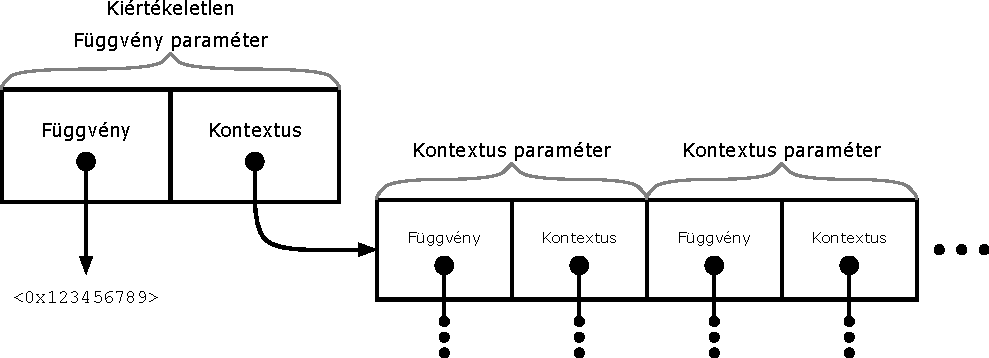
\includegraphics{fig/uneval-param.pdf}
            \caption{Kiértékeletlen függvény paraméter}\label{fig:c4-params}
        \end{subfigure}
        \vskip.64cm
        \begin{subfigure}{\linewidth}
            \hfil\resizebox*{5.324cm}{!}{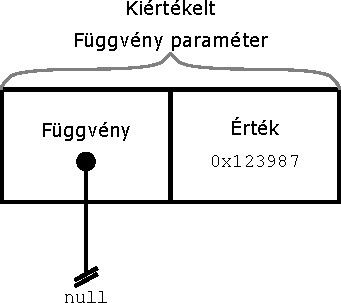
\includegraphics{fig/eval-param.pdf}}\hfil
            \caption{Kiértékelt függvény paraméter}\label{fig:c4-evaledparam}
        \end{subfigure}
        \caption{Paraméterek memóriabeli ábrázolása}
    \end{figure}

    Kiértékelés során csak egyszer kívánatos egy--egy paramétert kiszámolni, hogy a szemantikának megfelelő legyen a lefutás.
    Ehhez a kiértékelés után a következő lépéseket hajtja végre a hívott függvény (amelyik paramétere éppen kiértékelés alatt van).
    A kiértékelésből kapott értékekkel felülírja a második értéket a tömbben, majd, hogy a következő hívások esetén ismert legyen a paraméter kiértékelt volta, a függvény mutatóját \inlcode{null}ra állítja.
    \Aref{fig:c4-evaledparam}.~ábra ezt mutatja az állapotot be.
    Hogy ezt felismerje, minden hivatkozás elsőként az első paraméter nem \inlcode{null} értékét ellenőrzni, és aszerint vagy visszaadja az második értéket, vagy ha nem \inlcode{null}, akkor a megfelelő módon kiértékeli.

    \subsection{Closure blokkok}

    Egy blokk definiálásakor hivatkozhat egy olyan függvényre/változóra, amelyik a rajta kívüle eső blokkban lett definiálva, de nem globális.
    (Belátható, hogy csak globálisokra hivatkozáskor nincs semmi probléma.)
    Ilyenkor a számítás során szükség van arra az értékre, amelyik a hívás pillanatában érvényes.
    Az ilyen extra feltételekkel rendelkező blokkok az \un \gls{closure} blokkok.

    A megvalósításhoz a C4 szinten adott aritásnál egyel több paraméterük van: egy extra mutató paramétert kapnak a legelső pozícióban.
    Ebben ahány függvény fölött számítanak \gls{closure}nek, annyiszor két mező található.
    Ezek az értékek innentől megegyeznek a paraméterek átadásánál írtakkal.


    \printglossary[type=\acronymtype,title=Rövidítésjegyzék]
    \addcontentsline{toc}{chapter}{Rövidítésjegyzék}

    \printglossary
    \addcontentsline{toc}{chapter}{\glossaryname}

    \bibliography{blAST}
    \addcontentsline{toc}{chapter}{\bibname}

\end{document}